\documentclass[]{article}
\usepackage{lmodern}
\usepackage{amssymb,amsmath}
\usepackage{ifxetex,ifluatex}
\usepackage{fixltx2e} % provides \textsubscript
\ifnum 0\ifxetex 1\fi\ifluatex 1\fi=0 % if pdftex
  \usepackage[T1]{fontenc}
  \usepackage[utf8]{inputenc}
\else % if luatex or xelatex
  \ifxetex
    \usepackage{mathspec}
  \else
    \usepackage{fontspec}
  \fi
  \defaultfontfeatures{Ligatures=TeX,Scale=MatchLowercase}
\fi
% use upquote if available, for straight quotes in verbatim environments
\IfFileExists{upquote.sty}{\usepackage{upquote}}{}
% use microtype if available
\IfFileExists{microtype.sty}{%
\usepackage[]{microtype}
\UseMicrotypeSet[protrusion]{basicmath} % disable protrusion for tt fonts
}{}
\PassOptionsToPackage{hyphens}{url} % url is loaded by hyperref
\usepackage[unicode=true]{hyperref}
\hypersetup{
            pdfborder={0 0 0},
            breaklinks=true}
\urlstyle{same}  % don't use monospace font for urls
\usepackage{graphicx,grffile}
\makeatletter
\def\maxwidth{\ifdim\Gin@nat@width>\linewidth\linewidth\else\Gin@nat@width\fi}
\def\maxheight{\ifdim\Gin@nat@height>\textheight\textheight\else\Gin@nat@height\fi}
\makeatother
% Scale images if necessary, so that they will not overflow the page
% margins by default, and it is still possible to overwrite the defaults
% using explicit options in \includegraphics[width, height, ...]{}
\setkeys{Gin}{width=\maxwidth,height=\maxheight,keepaspectratio}
\IfFileExists{parskip.sty}{%
\usepackage{parskip}
}{% else
\setlength{\parindent}{0pt}
\setlength{\parskip}{6pt plus 2pt minus 1pt}
}
\setlength{\emergencystretch}{3em}  % prevent overfull lines
\providecommand{\tightlist}{%
  \setlength{\itemsep}{0pt}\setlength{\parskip}{0pt}}
\setcounter{secnumdepth}{0}
% Redefines (sub)paragraphs to behave more like sections
\ifx\paragraph\undefined\else
\let\oldparagraph\paragraph
\renewcommand{\paragraph}[1]{\oldparagraph{#1}\mbox{}}
\fi
\ifx\subparagraph\undefined\else
\let\oldsubparagraph\subparagraph
\renewcommand{\subparagraph}[1]{\oldsubparagraph{#1}\mbox{}}
\fi

% set default figure placement to htbp
\makeatletter
\def\fps@figure{htbp}
\makeatother


\date{}

\begin{document}

\section{معرفی}\label{ux645ux639ux631ux641ux6cc}

تیم برنامه نویسی عرش تقدیم میکند

\section{معرفی}\label{ux645ux639ux631ux641ux6cc-1}

تیم برنامه نویسی عرش تقدیم میکند

\section{راهنمای
بازی}\label{ux631ux627ux647ux646ux645ux627ux6cc-ux628ux627ux632ux6cc}

\begin{itemize}
\tightlist
\item
  \href{entergame.md}{ورود به بازی}
\item
  \href{enviroment.md}{معرفی محیط بازی}
\item
  \href{endgame.md}{پایان بازی}
\end{itemize}

\section{راهنمای ورود به
بازی}\label{ux631ux627ux647ux646ux645ux627ux6cc-ux648ux631ux648ux62f-ux628ux647-ux628ux627ux632ux6cc}

در صفحه آغازین بازی می توانید با انتخاب موضوع و زبان مورد نظر وارد بازی
شوید.

در قسمت ۱ می توانید موضوع مورد نظرات را انتخاب کنید

در قسمت ۲ و براساس زبان نوشته شده می توانید بازی را فارسی یا انگلیسی
بازی کنید

چون این آموزش بر مبنای زبان فارسی تهیه شده است ما بازی را بر اساس زبان
فارسی شروع میکنیم.

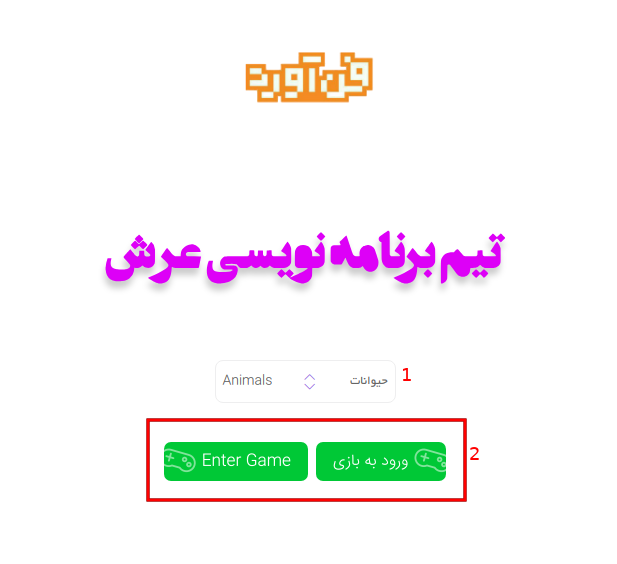
\includegraphics{../images/entergame.png}

\subsubsection{موضوع
کلمات}\label{ux645ux648ux636ux648ux639-ux6a9ux644ux645ux627ux62a}

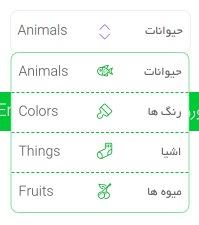
\includegraphics{../images/select-category.png}

\section{معرفی محیط
بازی}\label{ux645ux639ux631ux641ux6cc-ux645ux62dux6ccux637-ux628ux627ux632ux6cc}

همانطور که در تصویر مشاهده می کنید محیط بازی به ۶ قسمت تقسیم شده است:

\begin{enumerate}
\tightlist
\item
  ۱- موضوع کلمات انتخاب شده را نشونت می ده
\item
  ۲- کاراکتر بعدی که میاد رو نشون میده. میتونه کمک کننده باشه که چجوری
  کلمات رو بچینی
\item
  ۳- در ابتدا که وارد اینجا میشی بازی هنوز شروع نشدست. رو این دکمه کلیک
  کن تا بازی شروع بشه
\item
  ۴- بخش تنظیمات بازیه
\item
  ۵- وضعیت امتیاز، تعداد کلمات ساخته شده و مدت زمان طی شده رو بهت نشون
  میده
\item
  ۶- محیط اصلی بازی که در اون حروف میان و باید مرتبشون کنی
\end{enumerate}

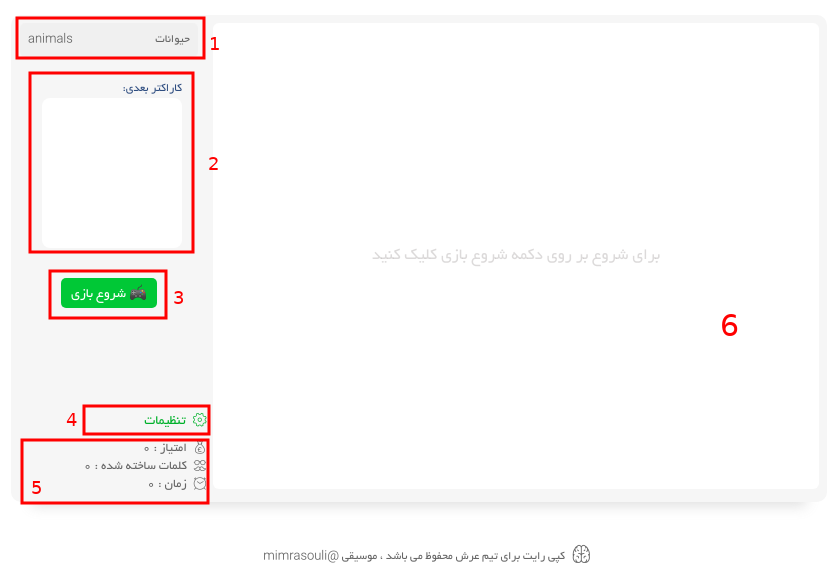
\includegraphics{../images/enviroment.png}

\section{موضوع
کلمات}\label{ux645ux648ux636ux648ux639-ux6a9ux644ux645ux627ux62a-1}

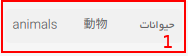
\includegraphics{../../assets/images/enviroments/1-category.png}

قبل از ورود به محیط بازی موضوع کلمات رو مشخصی میکنی و این بالا نشون داده
میشه. فعلا بازی دارای ۴ موضوع هست:

\begin{itemize}
\tightlist
\item
  حیوانات
\item
  رنگ ها
\item
  اشیا
\item
  میوه ها
\end{itemize}

\section{کاراکتر
بعدی}\label{ux6a9ux627ux631ux627ux6a9ux62aux631-ux628ux639ux62fux6cc}

در این قسمت کاراکتر بعدی که قراره برات بیاد نشون داده میشه. میتونه کمک
کنه تا استراتژی مناسبی داشته باشی و کلمات رو راحت تر کنار هم بچینی


\includegraphics{../../assets/images/enviroments/2-next-char.png}

\section{دکمه ها}\label{ux62fux6a9ux645ux647-ux647ux627}

\begin{itemize}
\item
  همون اول که میای تو بازی همه چی متوقفه تا با شرایط بازی اوکی تر بشی.
  برای اینکه شروع کنی بازیو رو دکمه
  
\includegraphics{../../assets/images/enviroments/3-buttons-start.png}
  کلیک کن تا بازی شروع بشه
\item
  وقتی بازی شروع شه دکمه سبز ``شروع بازی'' میره و جاش
  
\includegraphics{../../assets/images/enviroments/3-buttons-pause-restart.png}
  میاد. با کلیک روی ``توقف بازی'' بازی برات استپ میشه و با کلیک روی
  ``ریستارت بازی''، بازی دوباره از اول برات شروع میشه
\item
  وقتی روی ``توقف بازی'' کلیک کنی شکل دکمه ها
  
\includegraphics{../../assets/images/enviroments/3-buttons-resume-restart.png}
  میشه که با کلیک روی ``ادامه بازی'' میتونی بازی رو ادامه بدی
\end{itemize}

\section{تنظیمات}\label{ux62aux646ux638ux6ccux645ux627ux62a}

با کلیک روی

\includegraphics{../../assets/images/enviroments/4-settings.png} برات یک
پنجره به شکل زیر باز میشه که دارای بخش های مختلفیه. بعد از عکس برات
توضیح دادیم هر قسمتو

\begin{itemize}
\tightlist
\item
  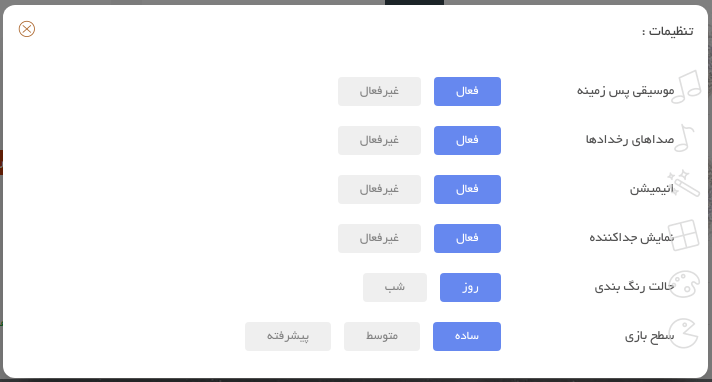
\includegraphics{../../assets/images/enviroments/4-settings-modal.png}
\end{itemize}

\paragraph{موسیقی پس
زمینه}\label{ux645ux648ux633ux6ccux642ux6cc-ux67eux633-ux632ux645ux6ccux646ux647}

موسیقی که موقع بازی کردن داره پخش میشه رو میتونی کنترل کنی

\emph{پیشفرض: فعال}

\paragraph{صداهای
رخدادها}\label{ux635ux62fux627ux647ux627ux6cc-ux631ux62eux62fux627ux62fux647ux627}

صدای پایین اومدن کلمات، حذف شدن کلمات جور شده و \ldots{} با این کنترل
میشه

\emph{پیشفرض: فعال}

\paragraph{انیمیشن}\label{ux627ux646ux6ccux645ux6ccux634ux646}

انیمیشن پایین آمدن کلمات، حذف کلمات جور شده و\ldots{}

\emph{پیشفرض: فعال}

\paragraph{نمایش جدا
کننده}\label{ux646ux645ux627ux6ccux634-ux62cux62fux627-ux6a9ux646ux646ux62fux647}

وقتی فعال باشه یک سری خطوط جدا کننده در محیط اصلی بازی نشون میده که
میتونه کمکت کنه تا راحت تر کلمات رو تراز کنی

\emph{پیشفرض: غیر فعال}

\begin{itemize}
\tightlist
\item
  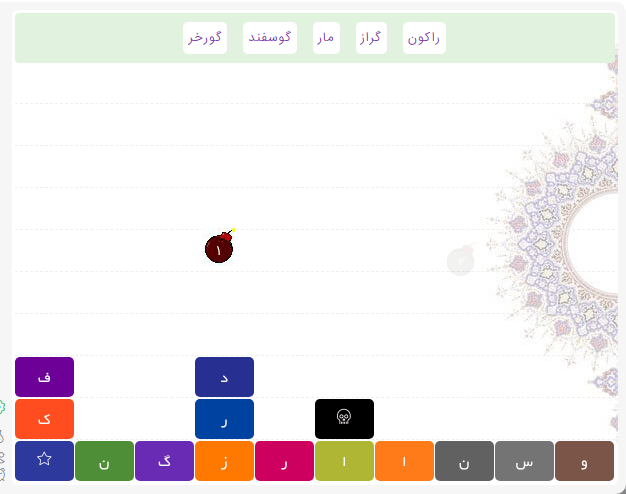
\includegraphics{../../assets/images/enviroments/4-settings-grid.png}
\end{itemize}

\paragraph{سطح بازی}\label{ux633ux637ux62d-ux628ux627ux632ux6cc}

جرئت داری سخت ترش کن !!!

\emph{پیشفرض: ساده گذاشتیم عادت کنی}

\section{وضعیت}\label{ux648ux636ux639ux6ccux62a}

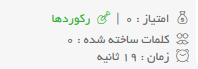
\includegraphics{../../assets/images/enviroments/5-status.png}

امتیاز کسب شده، تعداد کلمات ساخته شده و مدت زمان گذشته شده از بازی رو
بهت نشون میده

\begin{itemize}
\tightlist
\item
  فکر کنم توضیحات خاصی نیاز نباشه :)
\end{itemize}

\section{محیط اصلی
بازی}\label{ux645ux62dux6ccux637-ux627ux635ux644ux6cc-ux628ux627ux632ux6cc}

قسمت اصلی بازی که حروف میان و باید مرتبشون کنی

\begin{itemize}
\item
  برای بازی کردن با کامپیوتر از
  
\includegraphics{../../assets/images/arrow-keys.png} استفاده کن
\item
  برای موبایل هم کافیه روی صفحه swipe کنی
\item
  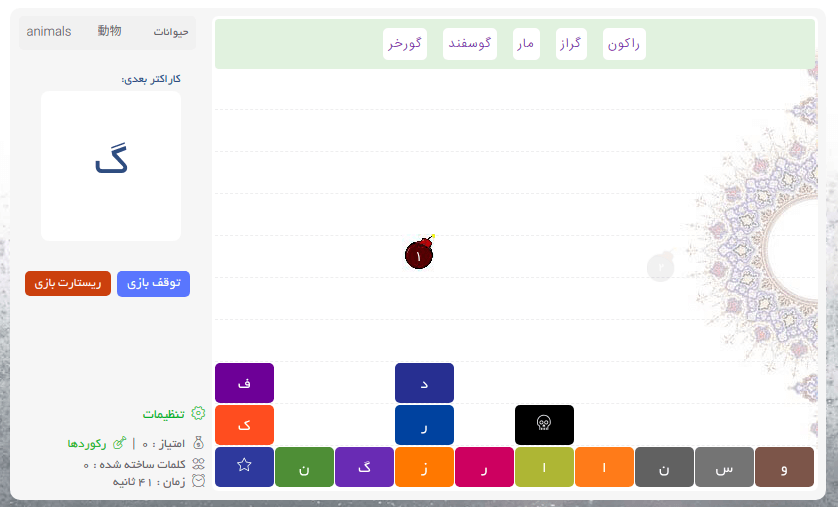
\includegraphics{../../assets/images/enviroments/6-main-game.png}
\end{itemize}

\section{پایان
بازی}\label{ux67eux627ux6ccux627ux646-ux628ux627ux632ux6cc}

این نیاز به داکیومنت داره هنووز

\begin{itemize}
\tightlist
\item
  پایان بازی به در دو صورت اتفاق میفته
\end{itemize}

\subsubsection{۱- رسیدن ستون بازی به
انتها}\label{ux631ux633ux6ccux62fux646-ux633ux62aux648ux646-ux628ux627ux632ux6cc-ux628ux647-ux627ux646ux62aux647ux627}

اگر تعداد حروف زیاد بشن و به از بالا تا پایین صفحه پر بشن اون وقت شما
بازنده میشی

\subsubsection{۲- تمام شدن کلمات دسته
بندی}\label{ux62aux645ux627ux645-ux634ux62fux646-ux6a9ux644ux645ux627ux62a-ux62fux633ux62aux647-ux628ux646ux62fux6cc}

\section{راهنمای
فنی}\label{ux631ux627ux647ux646ux645ux627ux6cc-ux641ux646ux6cc}

\section{راه اندازی برای
توسعه}\label{ux631ux627ux647-ux627ux646ux62fux627ux632ux6cc-ux628ux631ux627ux6cc-ux62aux648ux633ux639ux647}

\paragraph{گام اول}\label{ux6afux627ux645-ux627ux648ux644}

\begin{itemize}
\tightlist
\item
  ابتدا بنا به سیستم عاملتون \href{https://nodejs.org/en/}{Node.js} را
  نصب کنید.
\end{itemize}

\paragraph{گام دوم}\label{ux6afux627ux645-ux62fux648ux645}

\begin{itemize}
\tightlist
\item
  بعد از نصب \href{https://nodejs.org/en/}{Node.js} دستور زیر را در
  ترمینال وارد کنید.
\item
  \texttt{npm\ install\ -g\ yarn}
\end{itemize}

\paragraph{گام سوم}\label{ux6afux627ux645-ux633ux648ux645}

\begin{itemize}
\tightlist
\item
  به محل قرارگیری فایل های پروژه رفته و دستور زیر را در ترمینال بزنید.
\item
  \texttt{yarn}
\item
  منتظر بمانید تا همه ی پکیج ها نصب شوند
\end{itemize}

\paragraph{گام چهارم}\label{ux6afux627ux645-ux686ux647ux627ux631ux645}

\begin{itemize}
\tightlist
\item
  بعد از اتمام گام سوم دستور زیر را در ترمینال بزنید.
\item
  \texttt{yarn\ run\ dev}
\end{itemize}

تبریک!! حالا مرورگر باز شده و به ادیتور خود رفته و با هر تغییر به صورت
خودکار صفحه بارگزاری مجدد می شود

\paragraph{گام پنجم:
منتشر}\label{ux6afux627ux645-ux67eux646ux62cux645-ux645ux646ux62aux634ux631}

بعد از اینکه کارهای توسعه و غیره تمام شد و قصد انتشار برنامه را دارید
دستور زیر را در ترمینال جاری پروژه بزنید:

\begin{itemize}
\tightlist
\item
  \texttt{yarn\ run\ build}
\end{itemize}

فولدر ‍\texttt{dist} در محل پروژه ساخته شده که بهینه سازی شده است جهت
منتشر کردن. می توانید با آپلود این فولدر بر روی سرور رسما برنامه را
منتشر کنید

\section{ویرایش داکیومنت
gitbook}\label{ux648ux6ccux631ux627ux6ccux634-ux62fux627ux6a9ux6ccux648ux645ux646ux62a-gitbook}

این داکیومنت توسط
\href{https://github.com/GitbookIO/gitbook-cli}{gitbook-cli} نوشته شده
است. در صورتی که نیاز به تغییر دارد می توانید به طریق زیر عمل کنید

\paragraph{گام اول}\label{ux6afux627ux645-ux627ux648ux644-1}

یک ترمینال باز کنید و دستور زیر را وارد کنید.

\begin{itemize}
\tightlist
\item
  \texttt{npm\ install\ -g\ gitbook-cli}
\end{itemize}

\paragraph{گام دوم}\label{ux6afux627ux645-ux62fux648ux645-1}

به محل پروژه رفته و در فولدر \texttt{wiki} یک ترمینال باز کنید و دستور
زیر را بزنید:

\begin{itemize}
\tightlist
\item
  \texttt{gitbook\ install}
\end{itemize}

\subsubsection{گام سوم}\label{ux6afux627ux645-ux633ux648ux645-1}

سپس دستور زیر را بزنید:

\begin{itemize}
\tightlist
\item
  \texttt{gitbook\ serve} حال در یک ادیتور میتوانید فایل های مربوطه را
  ویرایش کرده و تغییرات را مشاهده کنید
\end{itemize}

\paragraph{گام چهارم:
منتشر}\label{ux6afux627ux645-ux686ux647ux627ux631ux645-ux645ux646ux62aux634ux631}

پس از تغییرات در صورتی که نیاز به انشار دارید دستور زیر را بزنید

\begin{itemize}
\tightlist
\item
  \texttt{gitbook\ build}
\end{itemize}

سپس محتوای فولدر \texttt{\_book} را در سرور آپلود کنید

\end{document}
